\documentclass[superscriptaddress,twocolumn,pre]{revtex4}

\usepackage{ifthen}
\newboolean{pnas}
\setboolean{pnas}{false}

\usepackage{amsmath}
\usepackage{amsfonts}
\usepackage{amssymb}
\usepackage{mathtools}
\usepackage{graphicx}
\usepackage[T1]{fontenc}
\usepackage[utf8]{inputenc}
\graphicspath{{images/}}
\usepackage{color}
\usepackage[pdfstartview=FitH,
            breaklinks=true,
            bookmarksopen=false,
            bookmarksnumbered=true,
            colorlinks=true,
            linkcolor=black,
            citecolor=black,
            urlcolor=black,
            pdftitle={Peptidome},
            pdfauthor={Andreas Mayer},
            pdfsubject={}
            ]{hyperref}
\newcommand{\B}{\boldsymbol}
\newcommand{\ud}{\mathrm{d}}
\newcommand{\<}{\langle}
\renewcommand{\>}{\rangle}

\def\(({\left(}
\def\)){\right)}                       
\def\[[{\left[}
\def\]]{\right]}

\newcommand{\AM}[1]{{\color{blue}#1}}

\begin{document}

\title{The statistical ensemble approach to immune discrimination}
%\author{Andreas Mayer}
%\author{Quentin Marcou}
%\author{Warren James}
%\author{Christopher Russo}
%\author{William Bialek*}
%\author{Benjamin D Greenbaum*}
\date{\today}

\begin{abstract}
The immune system needs to distinguish molecular features of pathogens from those found in the organisms' own proteins. A naive but universal way to discriminate, would be to have a system that can recognize any possible foreign peptide, while whitelisting every self peptide that should not elicit a reaction via negative selection. This previously prevailing view has been challenged in recent decades for the T cell system by experiments showing that many self-peptides are not entirely eliminated, but either do not make adequate antigens or are suppressed via regulatory mechanism and that T-cell receptors can be highly non-specific. The implication is that the immune system has adopted a different evolutionary strategy needs to be better understood. To begin to understand this approach we characterize the self and pathogen proteomes as statistical ensembles. Probabilistic models reveal how both universal and phyla-specific constraints on protein evolution shape the statistics of both proteomes. The models furthermore allow us to quantify to what extent the ensembles differ systematically, and hypothesize that the immune system has evolved to maximize the likelihood of recognition based on peptide statistics, since evolution is unlikely to develop strategies for organisms to combat pathogen features they never encounter. We analyze whether and how these differences might be used for an efficient immune defense. Finally, we compare predictions about what would be an efficient immune strategy to what is known about epitopes recognized by the immune system. 
\end{abstract}

\maketitle

\section{Introduction}

A key question in quantitative immunology is how the immune system distinguishes foreign antigens from self-antigens. There is one view of adaptive immunity in which both self and non-self antigens are random samples from a common (and essentially uniform) universe of peptides of a given length. Discrimination is then achieved solely on the basis of "white-listing": thymic negative selection acts to get rid of those T cells that are reactive to self, leaving everything else as a potentially recognizable foreign antigen. If the two types of antigens are instead drawn from different distributions, then some regions of peptide space will be much more likely to be self and some much more likely to be non-self. Over evolutionary timescales the recombination machinery could have evolved to bias the immune repertoire towards recognizing antigens that are more statistically unlikely to arise from the human proteome. Additionally due to different types of proteins and different types of environments, the amino acid and nucleic acid distributions needed for proper functioning of a protein might differ between a host and its pathogen. Alternatively, however, coevolution of pathogens with their hosts might select for pathogens that have a more similar distribution of peptides to their host than they would otherwise have by chance. The ability to address these issues experimentally has drastically changed our view of the T cell recognition machinery over the past decades \cite{Davis, garcia, crossreactivitypapers}. It is clear thymic selection eliminates self reactive T cells only partially. There are many self-reactive T cell in the blood that survive thymic selection, only to be suppressed by peripheral regulation. Moreover, T cell recognition is non-specific, as a cross-reactive T cell maybe be capable of recognizing many hundred peptides. It is therefore clear that self-peptides are eliminated only partially, likely in a biased manner, and that a cross reactive T-cell receptor repertoire may engage in negative selection only partially. 

The question of through what lens the immune system "sees" the world has renewed urgency in the context of cancer immunotherapy \cite{Luksza,Balachandran,Vonderheide}. As it has become clear that the immune system is capable of recognizing altered peptides in a tumor (referred to as neoantigens), which sort of antigens are more easily recognizable by the immune system has become a critical question. If there is a bias present in what makes a good antigen, this would aide in {\it in silico} predictions of response and the development of targets for next generation therapies. Here we revisit the often tacit assumptions about how evolution of the immune machinery might have shaped antigen prediction. In particular, there is a prevailing view of how detecting neoantigens is hard because they are often similar to self. If pathogens are generically very different from self then why would the immune system have evolved the capability of resolving small differences? We question that view by showing that the primary deviations away from a uniform distribution over oligiomers are shared between self and non-self peptides. That is, biases exist in both peptide and antigen distributions, but those biases are shard. If it is possible at all to evolve a system to discriminate small differences, than it seems plausible that efficient defense should focus on deviations from "more likely" regions, which the immune system can the statistics of from the self-proteome.

Previous immuno-peptidome analyses have focused on similarity between self and non-self peptides. Work by Claverie and co-workers \cite{Claverie1988} and later by Burroughs, De Boer, and Kesmir \cite{Burroughs2004} demonstrate that the number of shared nonamers decreases with evolutionary distance. The later work discusses some possible slight preference of the antigen processing pathway for non-self antigens. In a follow up work an overlapping set of authors build a tool for immunogenicity prediction based on small differences in amino acid usage in recognized epitopes \cite{Calis2013}, as well as discuss potential large holes created by self-tolerance \cite{Calis2012a}. A more recent follow up by Wortel et al. \cite{Wortel2018} shows that self and foreign peptides are largely similar (much more similar then words from different languages). They argue that under these conditions thymic selection should minimize the co-occurrence of similar self-peptides for efficient self/non-self discrimination based on negative selection. The emerging view would suggest that the immunogenicity of an antigen, via T cell reactivity, is related to how untypical it is given the normal distribution of the human proteome, rather than precision whitelisting. Recent works has found productivity in mutation derived neoantigen immunogenicity prediction both by incorporating distances to immunogenic viral peptides \cite{Luksza}, and distance from the self-proteome \cite{Vonderheide}. In cancer immunology \cite{Walz2015} it has also been known for sometime that immune activation can be achieved not just by neoantigens but also by large changes in protein abundance, such as those arising from epigenetic dysregulation. While mutation derived neoantigens have been implicated in response to checkpoint blockade immunotherapy, they are not the only source of immunogenicity \cite{XXX}. As such, bias towards unlikley peptides would account for both sequence and expression based discrimination.

Even a single proteome contains a great deal of data. The approximately 20000 genes times 1000 amino acids per gene on average gives $2 \cdot 10^7$ possible {\it k}-mer peptides, when not accounting restrictions on which can be processed and presented \cite{Luksza}. This also implies that most 5mers will still be represented in the proteome, as there are only about $20^5 = 3.2 \cdot 10^6$ possible 5mers. As a consequence, small changes in amino acid usage can lead to larger changes in the relative likelihood of longer stretches of otherwise random sequences: consider a 10\% difference for single amino acids than a random 8mer has a log-likelihood ratio of $1.1^8 \approx 2.15$. Even larger likelihood ratios are expected for long {\it k}-mers once pairwise or higher-order correlations are considered  \cite{Schneidman2006}. In that sense, the ability to capture features of genuine antigens would come from an adequate statistical model that captures typical self-peptides. Karlin and Bucher \cite{Karlin1992} have shown the existence of pairwise correlations in amino acid usage and discuss various structural reasons for these correlations. Peer et al. \cite{Peer2004} have shown that amino acid and oligopeptide compositions differentiate among phyla, which implies one can construct models of self-peptide that are not simply random, and follow up work has shown similar conclusions \cite{Bogatyreva2006}. On the other hand \cite{Lavelle2009} claim that generally 4mers and 5mers do not show large deviations from random models when taking care to remove bias by large protein families, implying the diversification of and selection upon these families account for most organism specific difference. On a more general level the question which structural constraints restrain the evolution of amino acid patterns has received attention for a long time \cite{Turjanski2018}. Random strings of amino acids do not yield valid, folding proteins, but amino acid strings of natural proteins are hard to distinguish from random, other than by deviations from uniform in individual amino acid frequencies that seem to be governed by amino acid mass \cite{BenAlbert}.

To capture these effects in an ensemble approach, we start by establishing an ensemble model of the self-proteome, demonstrating that most long peptides are random, other than single amino acid biases and a small amount of comparatively weak correlations. We build a maximum entropy distribution constrained to reproduce the amino acid frequencies and the correlations between pairs of amino acids a given distance apart (as we consider random substrings the distribution should only depend on absolute distance). A similar approach was done by Mora et al. \cite{Mora2010} for the distribution of antibodies, however antibodes offer greater antigen specificity than T-cell receptors. In doing so, we construct a theory of immune recognition whereby the species specific biases in the self-peptidome are leverage to find deviations from the self-distribution by pathogens. As pathogens, specifically viruses, have higher diversity that the self-proteome, yet need to interact with its internal machinery, we argue an immune model based on deviation from the "biased self", rather than trying to target pathogens uniformly and whitelisting, is optimal. 

\section{Results}


\subsection{Proteins are surprisingly random}

\begin{figure}
    \includegraphics{entropykmer}
    \caption{Entropy of the kmer distribution of the human and yeast proteome. The solid black line shows the maximal entropy of the flat distribution over the 20 possible amino acids $\log_2 20$. Note how the biggest reduction in entropy comes from amino acid biases with only a small further reduction by correlations in amino acid usage.
    \label{figentropykmer}
    }
\end{figure}


\begin{figure}
    \includegraphics[width=\columnwidth]{mutualinformationdecay}
    \caption{Mutual information between amino acids a certain distance apart in the human and mouse proteome. The mutual information is small as compared to the entropy of the single site $\sim 4$ bits, but extends to long distances. The prominent peaks at a distance that is a multiple of 28 amino acids in the human proteome are likely due to Zinc-finger repeats, more particularly C2H2 fingers (cf. high fold enrichments of cysteine and histdine at a distance of 28) \cite{Krishna2003}. 
    \label{figmutualinformationdecay}
    }
\end{figure}

How close to random is the protein distribution? To answer this question we calculate how much information about the amino acid in a certain position is revealed by knowing its neighbors. Concretely, we calculate the mutual information between amino acid pair a certain distance apart. The mutual information can be expressed as $I(X, Y) = H(X) + H(Y) - H(X, Y)$. We use this expression to calulate the mutual information from the single site entropies and the entropy of the joint distribution, which we calculate using the estimator proposed by Grassberger \cite{Grassberger2003}. (TODO: Use NSB estimator instead?) Note that one cannot assume uniform single site entropies across all comparions stemming most notably from differences in amino acid composition for the first few amino acids within a protein (Fig.~\ref{figentropyaa}). The universal constraints on unrelated proteins are surprisingly small as measured by the mutual information (Fig.~\ref{figmutualinformationdecay}, see also \cite{Lavelle2009}). 

\begin{figure}
    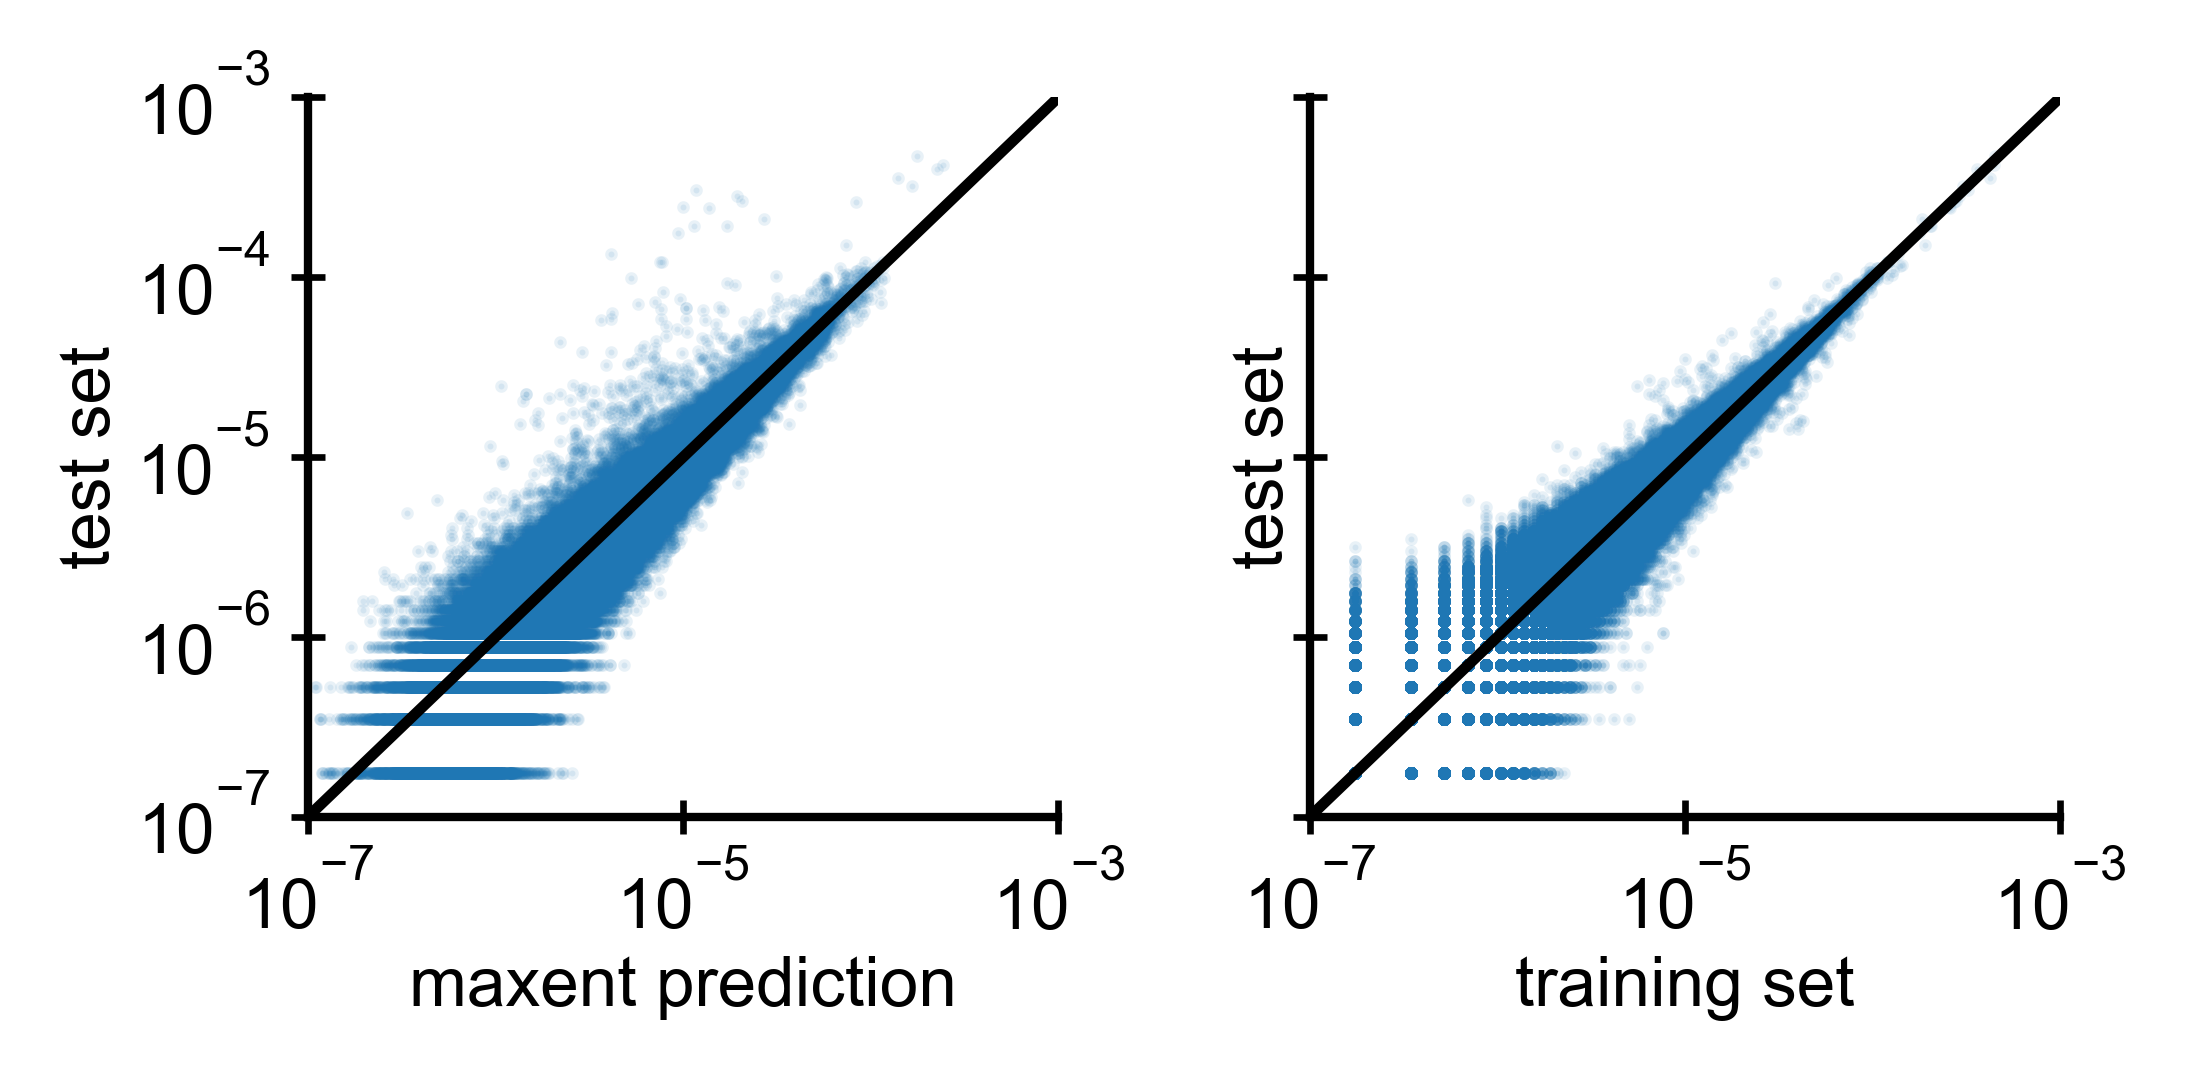
\includegraphics[width=\columnwidth]{4mer-comparison}
    \caption{Performance of the Maxent model for predicting the 4mer frequencies. Using an even split of the data into a test and a training set we compare predictions on the test set with the reproducibility of the frequencies between the training and test set.
    \label{fig4mermaxent}
    }
\end{figure}

\begin{table}
    \begin{center}
        \begin{tabular}{ c c }
            distribution & 4mer DKL\\ \hline
            uniform & 0.1115\\
            independent & 0.0195\\
            1st order Markov chain & 0.0132\\
            Pairwise Maxent & 0.0092\\
            2nd order Markov chain & 0.0087\\
            test & 0.0076\\
        \end{tabular}
    \end{center}
    \caption{Comparison of models based on 4mer frequencies}
\end{table}

We can further dissect which correlations between individual amino acids contribute to the mutual information. To do so we analyze the fold enrichment of amino acid doublets relative to an independent model. Most doublets are only over- or underrepresented moderately (Fig.~\ref{figdoubletentrichment}). An exception is a strong enrichment of Cysteine-Cysteine 3 amino acids apart. This enrichment has been found previously \cite{Greenbaum2014} and is likely due to a particular preference of cysteines to form disulfide bonds at this distance. Another prominent feature of this data are the relatively high enrichments along the diagonal at all distances. This might be attributable to amino acid repeats within some proteins \cite{Turjanski2018}.

\begin{figure}
    \includegraphics[width=\columnwidth]{doubletenrichment}
    \caption{Doublets are only enriched moderately relative to independent amino acid choice. (The enrichments are statistically significant, however. There are $\sim 10^7$ amino acids in the human proteome and thus on the order of $\sim 10^4$ counts per doublet. The relative error on the frequencies is thus on the order of only $\sim 1/\sqrt{10^4} = 10^{-2}$.)
    \label{figdoubletentrichment}
    }
\end{figure}

\subsection{The distribution of kmer likelihoods is close to being lognormal}

\begin{figure}
    \includegraphics{lognormalaa}
    \caption{Histogram of amino acid frequencies in the human proteome and lognormal approximation. (A) Probability density of the empirical likelihoods of a randomly drawn single amino acid and lognormal approximation. (B) Probability density of the empirical likelihoods of a randomly drawn 4-mer and lognormal prediction based on an independent model.
    (C) Probability density of the likelihoods of randomly drawn 9-mers under an independent model and lognormal prediction.
    \label{figlognormalaa}
    }
\end{figure}

As the two-point correlations are small we can try and approximate the likelihood of a given kmer in a proteome by an independent site model,
\begin{equation}
    P(s_1s_2 ... s_k) = \prod_{i=1}^k P(s_i),
\end{equation}
or more conveniently, their log-likelihood
\begin{equation}
    \ln P(s_1s_2 ... s_k) = \sum_{i=1}^k \ln P(s_i),
\end{equation}
which is a sum of independent random variables under the independent site model.
Using the central limit theorem we can approximate the distribution of the log-likelihoods of a kmer by a normal distribution. To do so we need to know the mean $\mu$ and variance $\sigma^2$ of the likelihood of a randomly picked amino acid. These can be calculated directly from the probability mass function of amino acid frequencies (Fig.~\ref{figlognormalaa}A). Note that the distribution of amino acid frequencies is somewhat skewed (skewness $\gamma_1 = -1.05$), but this skewness should diminish with $k$. The kmer distribution is approximately normal with mean $k \mu$ and variance $k \sigma^2$ as the cumulants of the sum of independent variables is equal to the sum of the cumulants.  Indeed, using the mean and variance of the distribution of frequencies of randomly chosen amino acids (Fig.~\ref{figlognormalaa}A), predicts relatively well the mean and variance of the empirical likelihoods of 4mers (Fig.~\ref{figlognormalaa}B) as well as of the model-based likelihoods of 9mers (Fig.~\ref{figlognormalaa}C). There are some deviations from the lognormal approximation apparent in both cases. There is a slight shift towards higher mean likelihoods, corresponding to a slightly reduced entropy in line with our earlier findings. Additionally, there are enrichments at the lower tail in both distributions, and the 4mer data shows an additional enrichment at the high likelihood tail.


\subsection{Quantifying differences between human and pathogen proteomes}

As argued above the dominant statistical bias away from a uniform peptide distribution arises from single amino acid biases. Therefore to start unraveling potential differences between human and pathogen proteomes we can quantify how much the distributions of single amino acids differs between proteomes. The overall differences can be quantified using the Kullback-Leibler divergence between the distribution of amino acid usage in a pathogen proteome and the human proteome. It turns out that these differences are small with some notable exceptions (Table~\ref{tabkldiv}). Interestingly, the parasite Plasmodium falciparum has the largest observed divergence from the human amino acid usage, which might be a result of the known AT bias of its genome \cite{Hamilton2017}. Vaccinia is higher than other viruses, which might attributable to it replicating outside the nucleus of the host cell using its own set of proteins for DNA replication and gene transcription \cite{Tolonen2001}. Mostly the Kullback-Leibler divergences between the doublet distributions are about twice the single site divergences. Notable exceptions are some of the viral proteomes, but this might be due to finite sampling effects biasing the entropy estimates for these small proteomes.

The Kullback-Leibler divergence is exactly the expected log-likelihood ratio drawing an amino acid from the pathogen distribution versus the human distribution. Under the independent model log-likelihoods are additive and thus the average log-likelihood ratio for a kmer is simply k times the calculated single site $D_{KL}$.
%In the limit of large $k$ 
%Chernoff-Stein Lemma!

%\begin{figure}
%    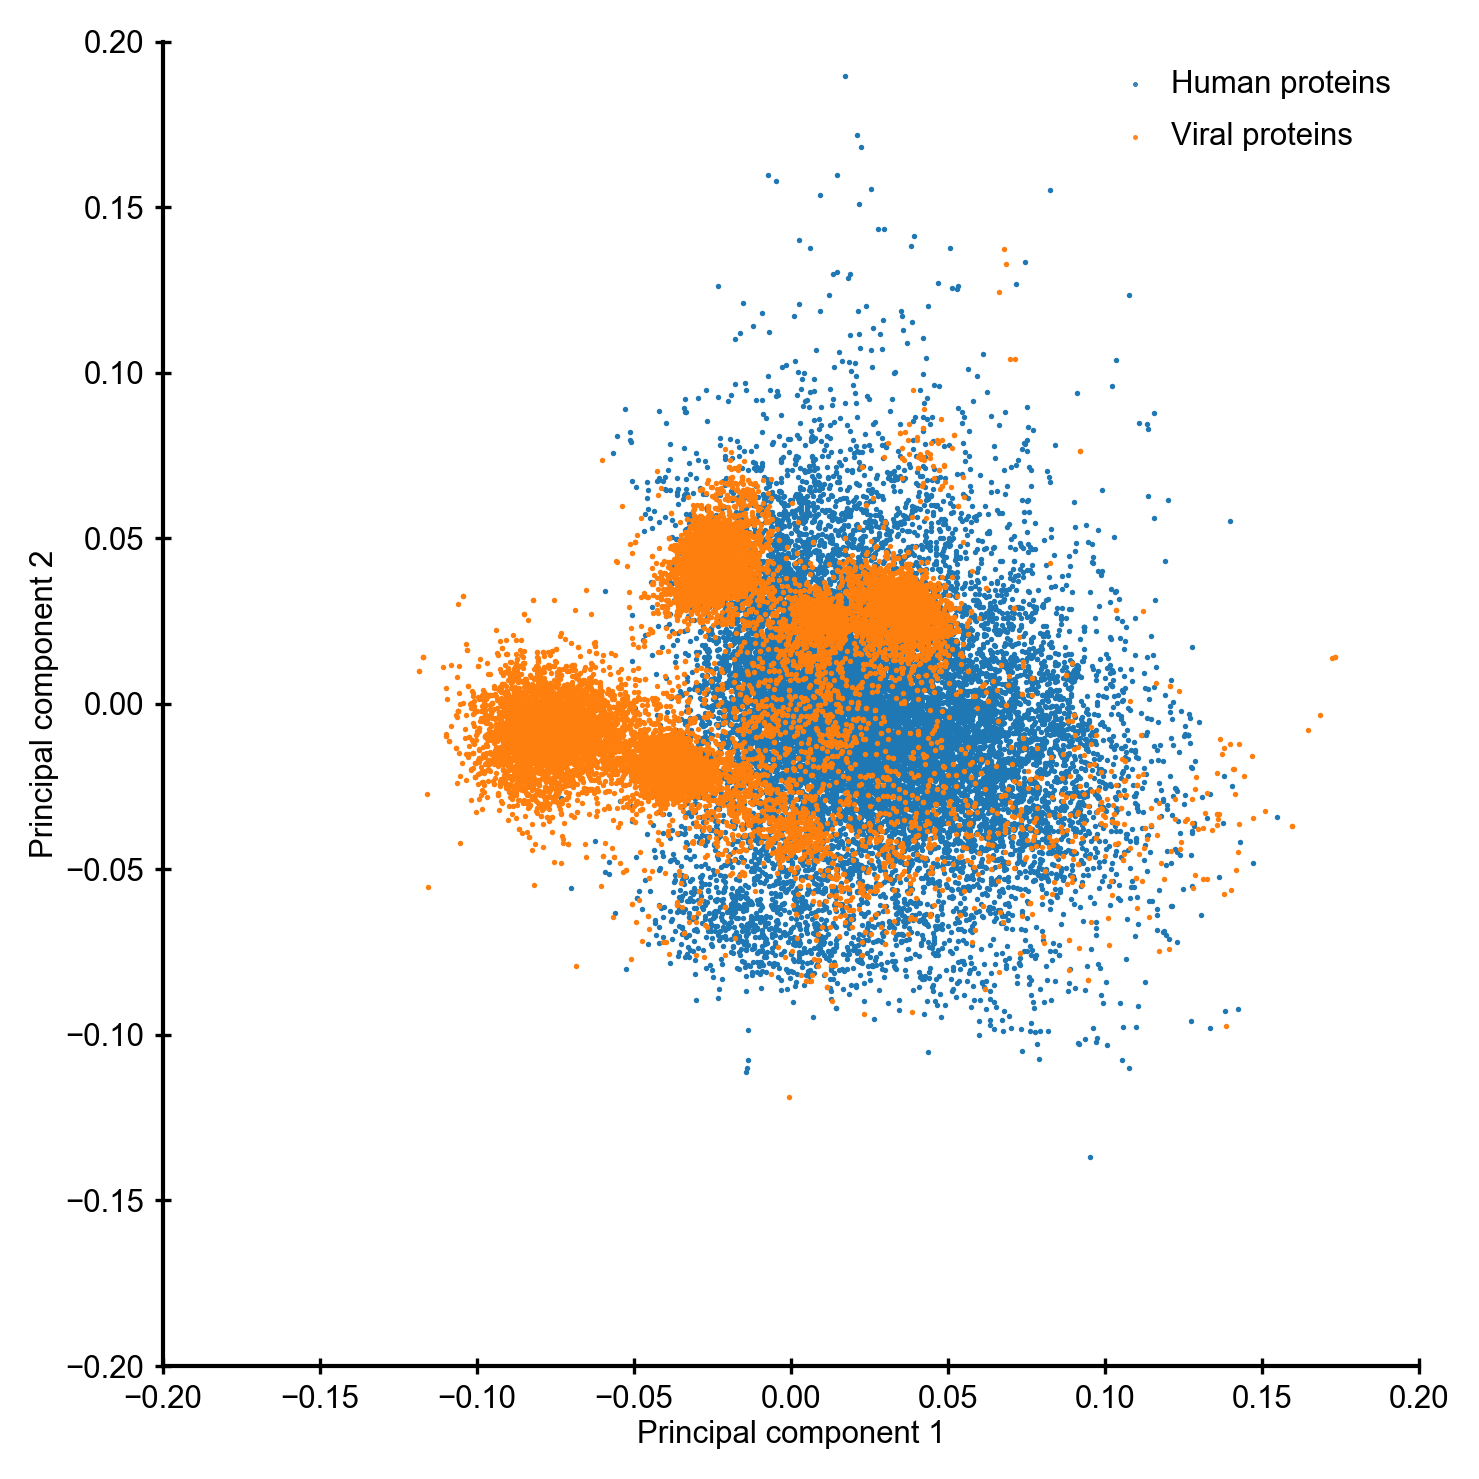
\includegraphics[width=\columnwidth]{viruses}
%    \caption{Likelihood of randomly drawn viral 9mers given a triplet model based on the human proteome statistics. B cell and T cell epitope likelihoods. Interestingly the B cell epitopes are more similar to the human proteome than if they where drawn at random.
%    \label{figviruses}
%    }
%\end{figure}

\subsection{A mathematical framework to model peptide statistics} 

The distribution $P(\B \sigma)$ of all possible peptides $\B \sigma$ within an organism is highly undersampled for even moderate length peptides. Still we can pursue a statistical approach and assign a probability to each peptide that measures how likely such a peptide is on average given the underlying proteome statistics.

We constrain some statistical observables $\langle f_\mu(\boldsymbol \sigma)\rangle$ to be equal to their empirical values $\bar{f_\mu}$, while otherwise keeping the probability distribution as random as possible. In mathematical terms this means that we are looking for the probability distribution that maximizizes the Shannon entropy
\begin{equation}
    S[P(\B \sigma)] = - \sum_{\B \sigma} P(\B \sigma) \log P(\B \sigma),
\end{equation}
subject to a normalization constraint and a constraint
\begin{equation}
    \langle f_\mu(\boldsymbol \sigma)\rangle = \sum_{\boldsymbol \sigma} P(\boldsymbol \sigma) f_\mu(\boldsymbol \sigma) = \bar{f_\mu},
\end{equation}
for each observable.
The optimization with respect to the normalization constraint can be performed analytically, which yields a Boltzmann distribution of the following form
\begin{equation}
    P(\boldsymbol \sigma) = \frac{1}{Z} \exp\left[ -E(\B \sigma) \right].
\end{equation}
with 
\begin{equation}
 E(\B \sigma) = \sum_{\mu=1}^K \lambda_\mu f_\mu(\boldsymbol \sigma)
\end{equation}
and 
\begin{equation}
    Z = \sum_{\B \sigma} \exp \left[ - E(\B \sigma) \right]
\end{equation}
    is a normalization factor, called the partition function in statistical mechanics.
We fit the model parameters using Boltzmann machine learning. To do so we estimate $\langle f_\mu(\B \sigma)\rangle$ using Monte Carlo methods for given model parameters. The parameters are then updated by gradient ascent,
\begin{equation}
    \lambda_\mu^{t+1} = \lambda_\mu^t + \epsilon_\mu^t \left(\langle f_\mu \rangle  - \bar{f_\mu}\right),
\end{equation}
where $\epsilon_\mu^t$ represents a learning rate (which generally can be coordinate dependent and time-varying).


\begin{figure*}
    \includegraphics[width=\textwidth]{maxent_freqs}
    \caption{Connected correlation functions of a maximum entropy model based on 1 and 2-point frequencies ressemble those of the training test set (upper row) within the training and test set error (lower row). Color indicates local density in regions with overplotting.
    \label{figmaxent_freqs}
    }
\end{figure*}

A common choice is to constrain the one and two-point frequencies
\begin{align}
    f_i^\alpha(\B \sigma) &= \sigma_i^\alpha, \\
    f_{ij}^{\alpha\beta}(\B \sigma) &= \sigma_i^\alpha \sigma_j^\beta,
\end{align}
where $\sigma_i^\alpha = 1$ if the amino acid at site i is of type $\alpha$ and zero otherwise.
This leads to a maximum entropy probability distribution that takes the form of a disordered Potts model,
\begin{equation}
    E(\boldsymbol \sigma) = - \sum_{i=1}^L \sum_{\alpha = 1}^{20} h_i^\alpha \sigma_i^\alpha - \sum_{i<j}^L \sum_{\alpha,\beta = 1}^{20} J_{ij}^{\alpha \beta}  \sigma_i^\alpha \sigma_j^\beta.
\end{equation}
The fitted model reproduces the 1- and 2-point connected correlations indicating fit convergence (Fig.~\ref{figmaxent_freqs}A,B). The model predicted connected third order correlations follow a similar trend between model and data, but are generally underestimated (Fig.~\ref{figmaxent_freqs}C).


\begin{figure*}
    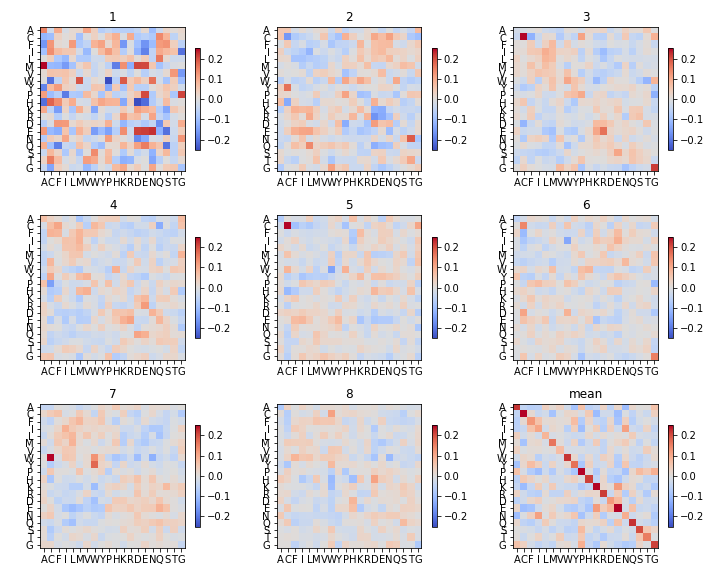
\includegraphics[width=\textwidth]{Jij_vs_dist}
    \caption{Mean coupling and deviations from mean coupling at a given distance. 
    \label{figJij_vs_dist}
    }
\end{figure*}


\begin{figure*}
    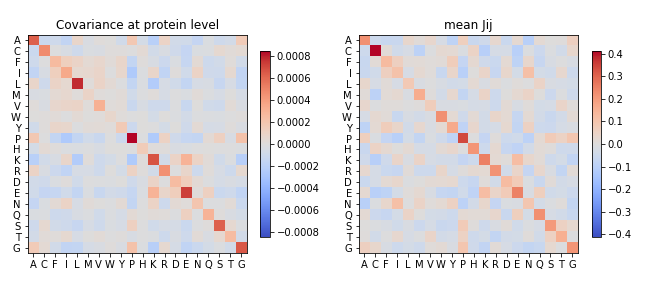
\includegraphics[width=\textwidth]{meanJij_aacovariance}
    \caption{Mean coupling matrix and covariance matrix between amino acid composition at protein level.
    \label{figJij_aacovariance}
    }
\end{figure*}


\begin{figure*}
    \includegraphics[width=\textwidth]{maxent_freqs_global}
    \caption{Correlation between compositional Maxent model and test set (upper row) and training and test set (lower row) for the first three connected correlation functions.
    \label{figmaxent_freqs_global}
    }
\end{figure*}

Given that many biases are compositional in nature we can also consider a simpler model that only involves a global constraint on the covariation of the total count of amino acids of different types:
\begin{align}
    n^\alpha(\B \sigma) &= \sum_i \sigma_i^\alpha, \\
    n^{\alpha\beta}(\B \sigma) &= n^\alpha(\B \sigma) n^\beta(\B\sigma) = \left(\sum_{i=1}^L \sigma_i^\alpha\right) \left(\sum_{j=1}^L \sigma_j^\beta\right).
\end{align}
This leads to a maximum entropy probability distribution that takes the form
\begin{equation}
    E(\boldsymbol \sigma) = - \sum_{\alpha=1}^{20} h^\alpha n^\alpha -  \sum_{\alpha,\beta = 1}^{20} J^{\alpha \beta} n^\alpha n^\beta,
\end{equation}
i.e. a model that only involves global couplings between amino acids independent of their distance.
A model with such global couplings captures a large fraction of 2-point correlations (Fig.~\ref{figmaxent_freqs_global}B), in line with the expectation that many of the constraints on amino acid covariation reflect compositional differences between different classes of proteins.


\begin{figure*}
    \includegraphics{dos}
    \caption{Density of states with respect to the 2-point model energy function for kmers from the test set and model-drawn kmers.
    \label{figdos}
    }
\end{figure*}

\begin{figure}
    \includegraphics[width=\columnwidth]{hammingdist}
    \caption{Distribution of Hamming distances between random pairs of sequences from the model and the test set normalized by expectation from comparison of training and test set sequences. The observed dip at small distances reveals further structure not captured by any of the models.
    \label{fighammingdist}
    }
\end{figure}



Once we have fitted the model parameters we can calculate the entropy of the distribution $P(\B \sigma)$. To do so we use the identity
\begin{align}
    S &= - \sum_{\B \sigma}  P(\B \sigma) \log P(\B \sigma),  \\
      &= \langle E(\B \sigma) \rangle - F, \quad F = - \log Z.
\end{align}
The mean energy can be calculated directly from Monte Carlo samples. To calculate the free energy we use thermodynamic integration as follows \cite{Marchi2019b}: We express the energy with respect to a reference energy $E_{ref}(\B \sigma)$ as $E(\B \sigma) = E_{ref}(\B \sigma) + \Delta E(\B\sigma)$, where the reference energy is choosen such that $F_{ref}$ can be calculated analytically. We define the perturbed energy function
\begin{equation}
    E_\alpha(\B \sigma) = E_{ref}(\B \sigma) + \alpha \Delta E(\B\sigma),
\end{equation}
which scales the contribution of the energy beyond the reference model.
To obtain the free energy we use the identity
\begin{equation}
    F(1) = F_{ref} + \int_0^1 \ud \alpha F'(\alpha).
\end{equation}
Note that
\begin{equation}
    F'(\alpha) = - \langle \Delta E(\B \sigma) \rangle_{\alpha},
\end{equation}
which allows us to approximate the integrand by Monte Carlo simulations. We numerically evaluate $F'(\alpha)$ for evenly spaced $\alpha \in [0, 1]$ and calculate the integral by Simpson's rule. Calculating the entropy in this way allows us to determine the reduction in the effective diversity in sequences implied by including different constraints (Fig.~\ref{figdiversity_reduction}). 

\begin{figure}
    \includegraphics{diversity_reduction}
    \caption{Effective diversity of modelled distributions of 9-mers including different constraints.
    \label{figdiversity_reduction}
    }
\end{figure}









\subsection{Features of immune epitopes}

\begin{figure}
    \includegraphics[width=\columnwidth]{likelihoodprofile-iedb-tcell}
    \caption{Likelihood of IEDB T cell epitopes given a triplet model based on the human proteome statistics compared to random self peptides. The three distributions are largely indistinguishable except for a slight depletion of epitopes at the highest likelihoods.
    \label{figtcelliedb}
    }
\end{figure}

Which of the possible peptides do eventually get recognized by the immune system? To answer this question we score known immune epitopes from the Immune Epitope Database (IEDB) against a model for the likeliehood of self peptides (Fig.~\ref{figtcelliedb}). There are few epitopes that are very likely under the self statistics, but overall the distributions are largely indistinguishable. There are also no statistical differences between IEDB entries with positive vs. negative assays.

We can zoom into epitopes from particular pathogens to see whether this finding is due to the similarity of the pathogen proteomes or to immune selection.



\subsection{A shell theory of immunogenicity?}

\begin{figure}
    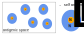
\includegraphics{shelltheorysketch}
    \caption{Sketch of the shell theory of immunogenicity: To be immunogenic an antigen needs to fall outside the tolerance region (orange), but within one of the detectable regions surrounding a self-antigen (blue).
    \label{figshelltheorysketch}
    }
\end{figure}

\begin{figure}
    \includegraphics[width=\columnwidth]{shelltheory}
    \caption{Immunogenicity as a function of the likelihood a peptide in the shell model. The probability of a peptide being immunogenic is defined as the probability of being detectable, but not tolerated. The probability of immunogenicity times the probability of peptides within the pathogen proteome (assumed to be lognormal with $mu = -1.25 k$ and $\sigma = 0.3 k$ with $k=9$) gives a hypothetical expected distribution for the epitopes, which is clipped at both ends.  
    \label{figshelltheory}
    }
\end{figure}

How likely is it that a peptide will be close enough to a self-peptide to be tolerized? How likely to be close enough such that there has been positive selection? To a first approximation neighboring peptides will have similar probabilities. Therefore the probabilities of a peptide relate to the local density and thus to the average distance to the nearest neighbor.

Consider that there is a number $N_T$ neighboring peptides that if they are in the self-peptidome would lead to tolerance, and a number $N_D > N_T$ of neighboring peptides that would lead to positive selection on TCRs recognizing the peptide and are thus needed for detectability. The probability of a peptide of probability $p$ being tolerized is $P_T \sim 1-(1-N_T p)^N$ assuming the $N$ possible self-peptides are sampled statistically independently from the peptidome distribution. As $N_T p \ll 1$ we can approximate $P_T \sim 1-e^{-N_T p N}$. Similarly, the probability of being detectable is $P_D \sim 1-(1-N_D p)^N \approx 1-e^{-N_D p N}$. Setting $N_T$ to the number of first neighbors (171 for 9mers), and $N_D$ to the number of second neighbors (25992 for 9mers) and assuming that $N$ is equal to the total possible number of kmers that can be generated from the full human proteome ($\sim 2 \cdot 10^7$), we can plot how $P_T$ and $P_D$ depends on $p$ (Fig.~\ref{figshelltheory}).

\bibliographystyle{apsrev}
\bibliography{library}

\begin{figure}
    \includegraphics{entropyaa}
    \caption{Entropy of the single site distribution of amino acids used in different positions along proteins in the human proteome. In an overwhelming majority of cases the first amino acid in a protein is a Methionine, because this amino acid is encoded by the start codon AUG. There is a slightly lower entropy o amino acids also in the following few amino acids, which might similarly be explained by known mRNA biases around the initiation codon (rf. Kozak consensus sequence). 
    \label{figentropyaa}
    }
\end{figure}


\section{An analysis of neighbor density in an independent site model}

\begin{figure}
    \includegraphics{nnproblikelihood}
    \caption{The nearest neighbor probability and the likelihood of a sequence are closely related. The likelihood of a 9mer drawn from an independent site model based on the human amino acid frequencies is closely related to the sum of the likelihoods of all its neighboring sequences. The deviation from a linear scaling is well desribed by the theory developed in the text. 
    \label{fignnproblikelihood}
    }
\end{figure}

When the probability is correlated across sequence space we expect sequences that are highly probable under a given model to also have more neighbors in a set of sequences drawn from that same model. Here we will make this link quantitative for an indepndent site model.

We denote by $k$ the length of the sequences $\B \sigma$ we consider and by $S$ the number of possible choices per site (e.g. for peptides we have $S=20$ amino acids). We do not impose that the model is translation invariant, i.e. the probability of an amino acid can depend on position,
\begin{equation} \label{eqpsigma}
    p(\B \sigma) = \prod_{i=1}^k p_i(\sigma_i).
\end{equation}
Let us define the probability that a randomly drawn sequence is a neighbor of sequence $\B \sigma$ as
\begin{equation}
    n(\B \sigma) = \sum_{\B \sigma' \sim \B \sigma} p(\B \sigma').
\end{equation}
We have 
\begin{align*}
    n(\B \sigma) &= \sum_{i=1}^k \sum_{s / \sigma_i} p(\B \sigma) \frac{p_i(s)}{p_i(\sigma_i)} \\
              &= p(\B \sigma) \sum_i \frac{1-p_i(\sigma_i)}{p_i(\sigma_i)}
\end{align*}
from which we finally obtain
\begin{equation}
    n(\B \sigma) = p(\B \sigma) \left[\sum_i \frac{1}{p_i(\sigma_i)} - k\right].
\end{equation}
Expanding $p_i(\sigma_i) = 1/S + \delta p_i(\sigma_i)$ around its mean value $1/S$ we obtain at first order
\begin{equation} \label{eqnsigmadeltas}
    n(\B \sigma) \approx p(\B \sigma) \left[ k (S-1) - S^2 \sum_i \delta p_i(\sigma_i)\right].
\end{equation}
We can rewrite Eq.~\ref{eqpsigma} as
\begin{align}
    p(\B \sigma) &= \prod_{i=1}^k \left(\frac{1}{S} + \delta p_i(\sigma_i) \right)
                 &= \frac{1}{S^k} e^{\sum_{i=1}^k \ln(1+ S \delta p_i(\sigma_i))}
\end{align}
and then expand similarly for small $\delta p_i$ to obtain
\begin{equation}
    p(\B \sigma) \approx \frac{1}{S^k} e^{S \sum_{i=1}^k \delta p_i(\sigma_i)}.
\end{equation}
The previous equation can be rewritten as
\begin{equation*}
    S \sum_{i=1}^k \delta p_i(\sigma_i) \approx \ln\left(p(\B \sigma)/p_0\right),
\end{equation*}
where $p_0 = 1/S^k$ is the average probability of a sequence.
Plugging this into Eq.~\ref{eqnsigmadeltas} yields
\begin{equation} 
    n(\B \sigma) \approx p(\B \sigma) \left[ k (S-1) - S \ln\left(p(\B \sigma)/p_0\right)\right].
\end{equation}

Note that this formula recovers the correct limiting behavior as $p(\B \sigma) \to p_0$, for which $n(\B \sigma)$ is simply the number of neighbors times the probability of a sequence. The formula shows that the density is locally proportional to the probability with a slope that varies slowly with the probability. On a log-log plot the slope is given by
\begin{equation}
\frac{\ud \ln n(\B \sigma)}{\ud \ln p(\B \sigma)} = 1 - \frac{S}{k(S-1) - S \ln(p(\B \sigma)/p_0)},
\end{equation}
which can be approximated as long as $p(\B \sigma)$ is within a factor of $k$ of $p_0$ as
\begin{equation}
\frac{\ud \ln n(\B \sigma)}{\ud \ln p(\B \sigma)} = 1 - \frac{S}{k(S-1)}.
\end{equation}

We can use the result derived earlier to calculate the probability 
\begin{align}
\bar n = \sum_{\B \sigma, \B \sigma', \B \sigma \sim \B \sigma'} p(\B \sigma) p(\B \sigma') 
\end{align}
with which two randomly chosen sequences are neighbors. We can rewrite
\begin{align*}
\bar n &= \sum_{\sigma} p(\B \sigma) \sum_{\sigma' \sim \sigma} p(\B \sigma')  \\
    &= \sum_{\B \sigma} p(\B \sigma) n(\B \sigma)\\
    &= 1/p_0 \sum_{\B \sigma} p_0 p(\B \sigma) n(\B \sigma) = 1/p_0 \langle p(\B \sigma) n(\B \sigma) \rangle,
\end{align*}
where the expectation value is taken with respect to the uniform distribution.
Plugging in Eq.~\ref{eqnsigmadeltas} we have
\begin{equation}
\bar n p_0 = \langle p(\B \sigma)^2 \rangle k(S-1) - S \langle p(\B \sigma)^2 \ln (p(\B \sigma)/p_0) \rangle.
\end{equation}
Up to second order we have
\begin{equation}
\langle p(\B \sigma)^2 \ln (p(\B \sigma)/p_0) \rangle \approx \frac{3}{2} \langle \delta p^2\rangle.
\end{equation}
Together with $\langle p^2 \rangle = \langle \delta p^2\rangle + p_0^2$ this yields the following relation between the average density and the coefficient of variation of $p$,
\begin{equation}
\bar n = p_0 k (S-1) \left[1+\langle \delta p^2/p_0^2 \rangle \left(1 - \frac{3S}{2k(S-1)}\right) \right]
\end{equation}





\begin{table}
    \begin{center}
        \begin{tabular}{ c c c }
            Organism&site $D_{KL}$&doublet $D_{KL}$\\
            \hline
Mouse&0.00023&0.00089\\
Yeast&0.046&0.097\\
Cockroach&0.015&0.033\\
Cattle&0.00031&0.0011\\
Chicken&0.0011&0.0038\\
Wheat&0.012&0.029\\
Soybean&0.013&0.033\\\hline
Vaccinia&0.13&0.27\\
InfluenzaB&0.043&0.17\\
InfluenzaA&0.042&0.17\\
CMV&0.035&0.085\\
HCV&0.064&0.2\\
HBV&0.078&0.28\\
DENV&0.049&0.19\\
HIV&0.043&0.19\\
EBV&0.043&0.1\\ \hline
Human viruses&0.015&0.038\\\hline
Ebola&0.023&0.12\\
Tuberculosis&0.11&0.23\\
Listeria&0.071&0.15\\
Burkholderia&0.1&0.23\\
Meningococcus&0.039&0.1\\
StreptococcusPyogenes&0.06&0.14\\
Hpylori&0.077&0.19\\
Lyme&0.19&0.38\\
Tetanus&0.15&0.3\\ 
Leprosy&0.077&0.17\\ \hline
Malaria&0.36&0.71\\
Chagas&0.017&0.051\\
OnchocercaVolvulus&0.03&0.069\\
        \end{tabular}
    \end{center}
    \caption{Kullback-Leibler divergence between amino acid frequencies (and doublet frequencies) in various proteomes and the human proteome (in bits). Human viruses: all viruses with human host from uniprot filtered for duplicates using the Uniref 90 criteria.}
    \label{tabkldiv}
\end{table}



\end{document}
